\section{Design}
\label{sec:design}

The system, \system{}, is based on Vizdom~\cite{vizdom} and addresses the aforementioned challenges, namely,
\begin{itemize*}
    \item To formulate hypotheses via user interaction;
    \item To visualize the statistical significance and other contextual information for each observation;
    \item To control multiple hypotheses dynamically in exploration;
    \item To progressively compute the risk of false discovery.
\end{itemize*}

\subsection{User Interface}
\label{sec:ui}

\begin{figure}
\centering
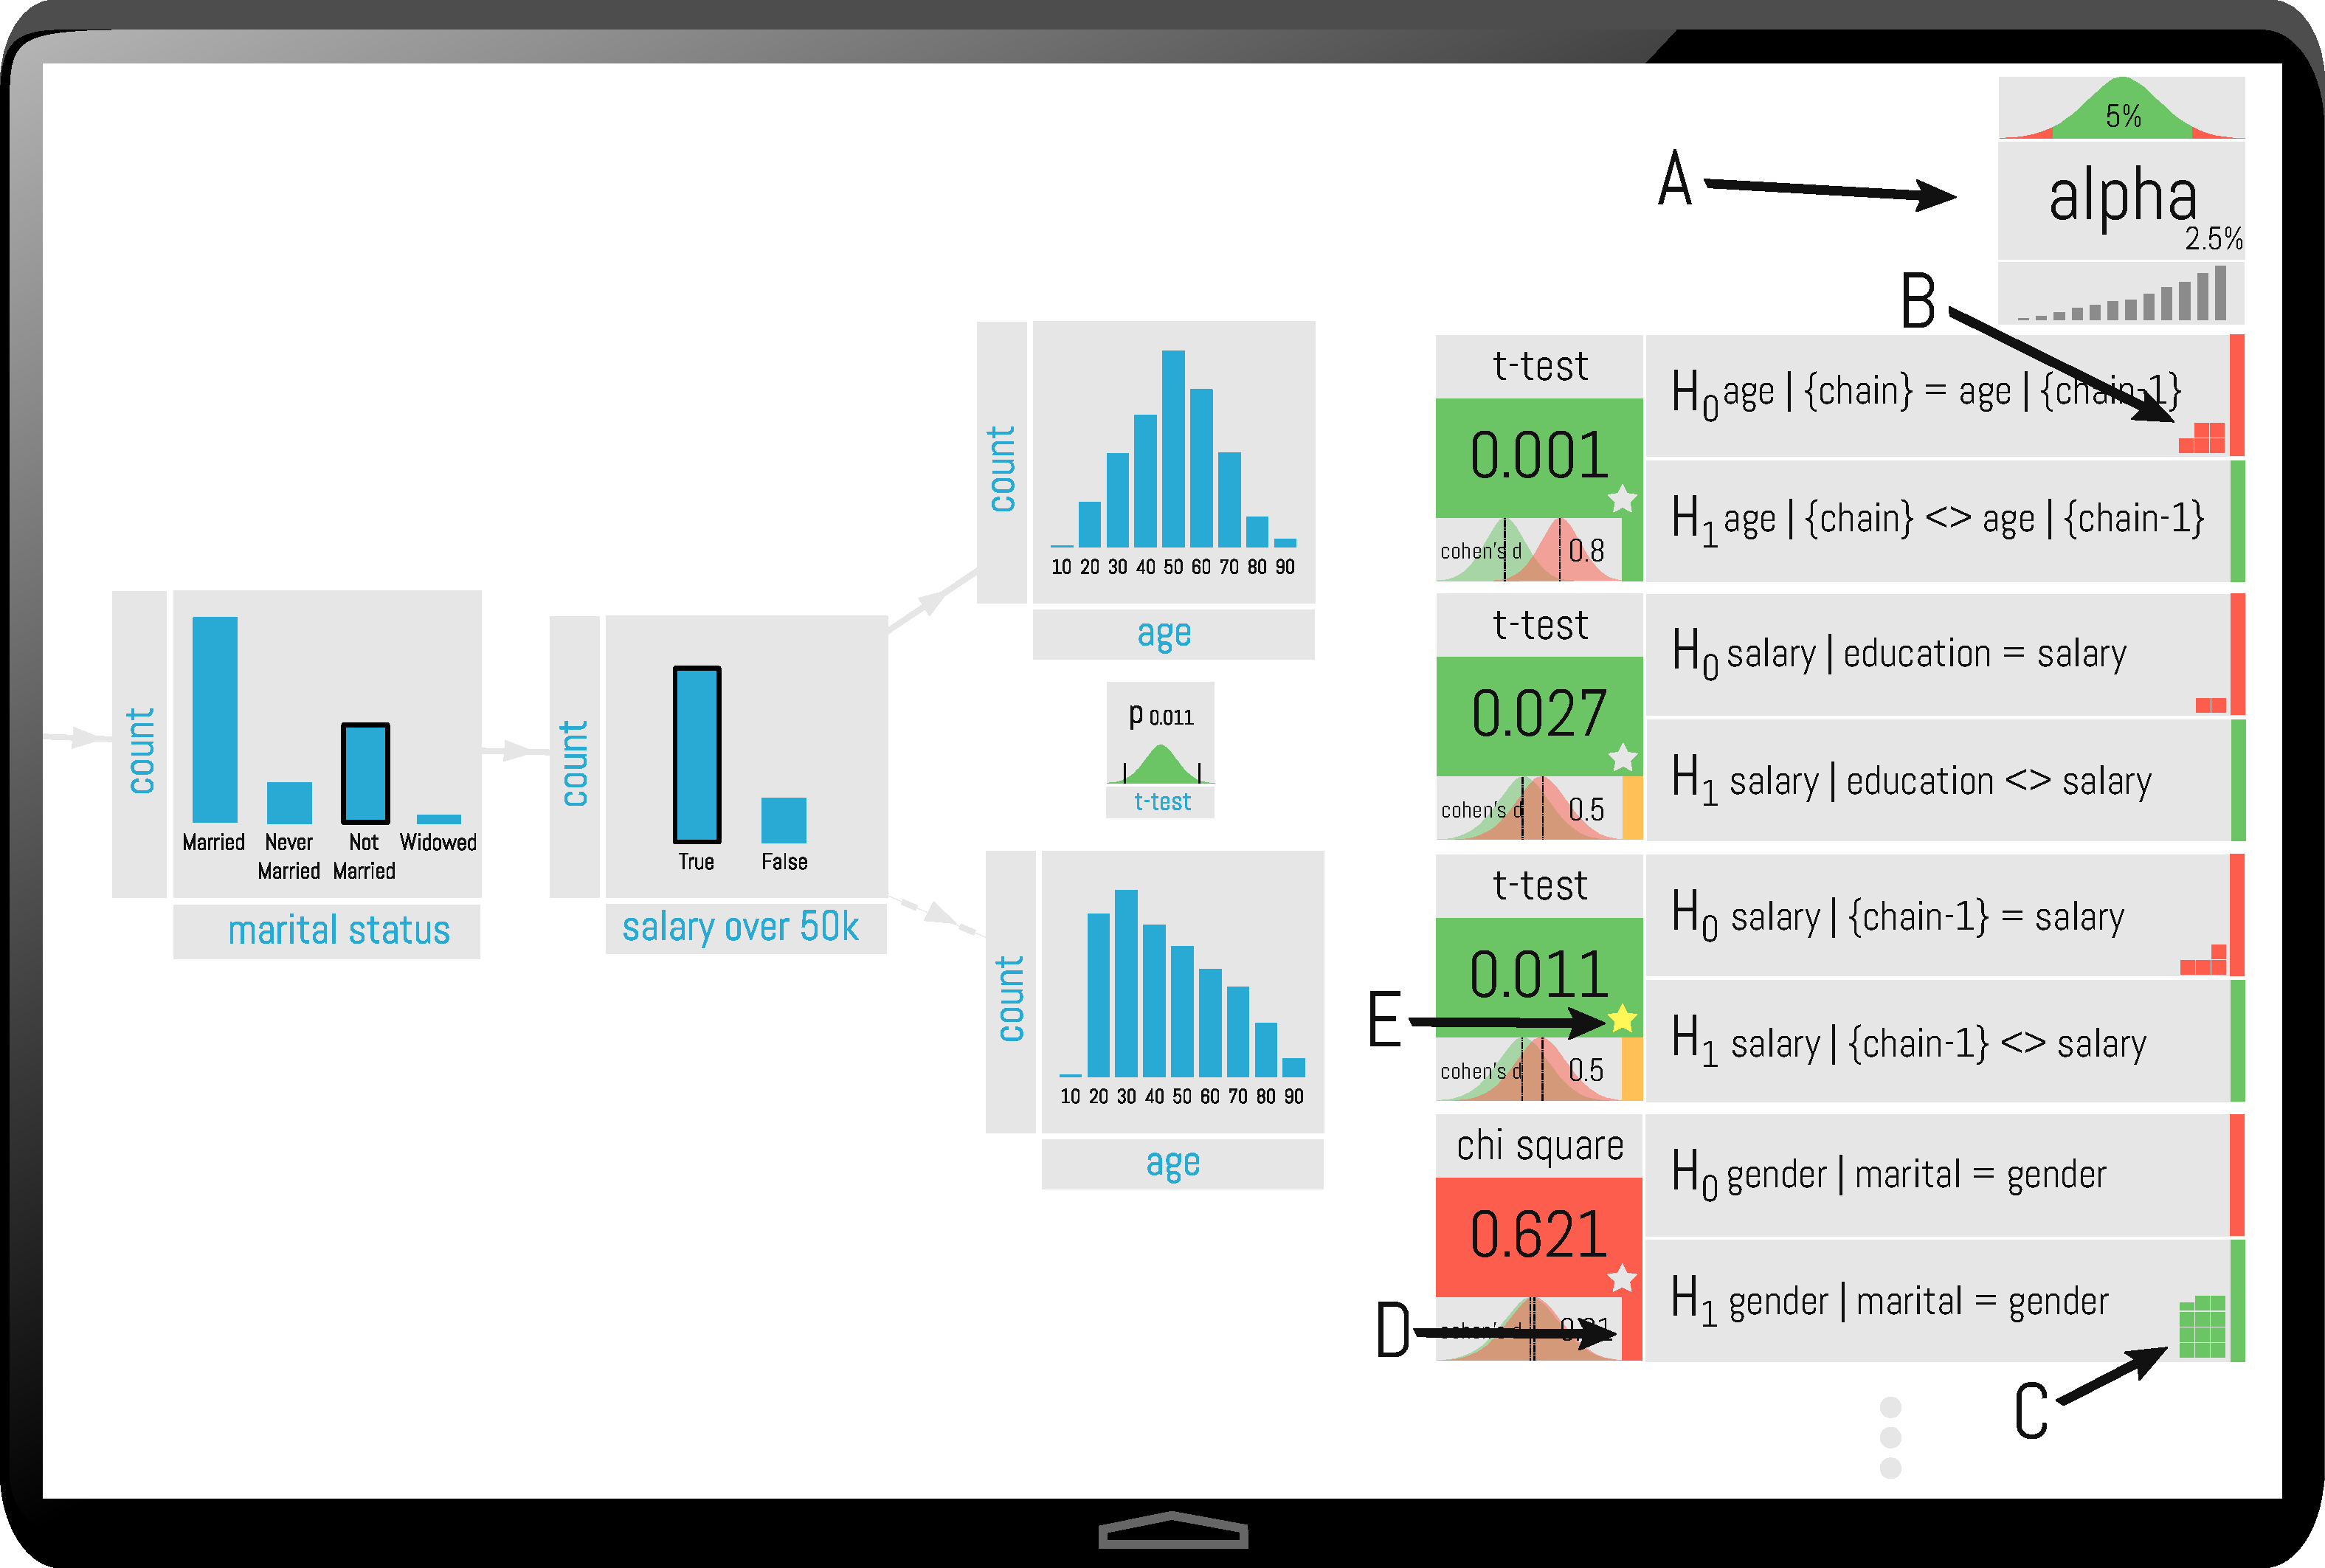
\includegraphics[width=0.47\textwidth]{figures/ui.pdf}
\caption{User interface design showing \system{}'s ``risk-gauge'' on the right which keeps track of all hypotheses and provides details for each of them.}
\label{fig:ui}	
\vspace{-4ex}
\end{figure}

\system{}'s user interface (UI) features an unbounded 2D canvas where visualizations can be laid out in a free form fashion (Figure~\ref{fig:ui}). It is based on our visual data exploration tool Vizdom~\cite{vizdom} but extended by three new features:

\textbf{Explicit and implicit hypothesis formulation:} For cases where users know which effect they want to statistically verify, we included support to explicitly create hypotheses through a gestural UI that poses minimal overhead to users.
Additionally however, we found that in many cases users do not deliberately think about chains of visualizations as tests even though users gain insights from them.  
For these instances, that we call implicit hypotheses, we augmented our system to formulate tests and display test results automatically. The class of tests we formulate automatically includes comparisons of subsets against the global population of a dataset such as the one illustrated in Figure \ref{fig:example}. The example shows a visualization chain where without an implicit hypothesis test (C), users might wrongly observe and perceive a significant effect (difference in bottom visualization between A and B).
% ez: maybe talk about the automatic test selection. 
% In other cases, where users either 
% However we ... 
 
\textbf{Visualization recommendations:} To speed up the potentially laborious process of manually exploring a dataset we added a visualization recommendation engine with false discovery control (Section~\ref{sec:backend}). Similar to SeeDB \cite{seedb} our \textit{recommender} allows users to search for filter conditions that have a significant effect (positive or negative) on a given reference visualization. We expose this functionality though a gestural touch UI that can be accessed from any visualization. 

\textbf{Hypotheses tracking:} A ``risk-gauge'' on the right-hand side of the display (A) serves two purposes, namely, to give user a summary of the multiple hypothesis correction procedure (e.g., in this case \ainv{} is used with a false discovery rate of 5\% and with current remaining budget of 70\%), and to provide access to a scrollable list of all the hypotheses that have been explored.
Each list entry can be expanded (in the example all are expanded) to display details about an observation and its statistical significance.  
The text labels describe the null and alternative hypotheses for each observation and the corresponding hypothesis test and \pval{}. Each color coded tile indicates whether the observation is statistically significant or insignificant, which corresponds to green or red respectively.  
The distributions of null and alternative hypotheses and the color coded effect size are also visualized (C).  
To help the user understand the effect of data collection, the sample size estimate for the current significance level is displayed for each hypothesis test assuming the effect size is fixed (B).  
For example, the five green squares in (B) indicates approximately five times the current data size with the same effect size would make this observation significant.
Finally, important insights can be marked by tapping the ``star'' icons (D).

\subsection{Backend}
\label{sec:backend}

\begin{figure}[!ht]
\centering
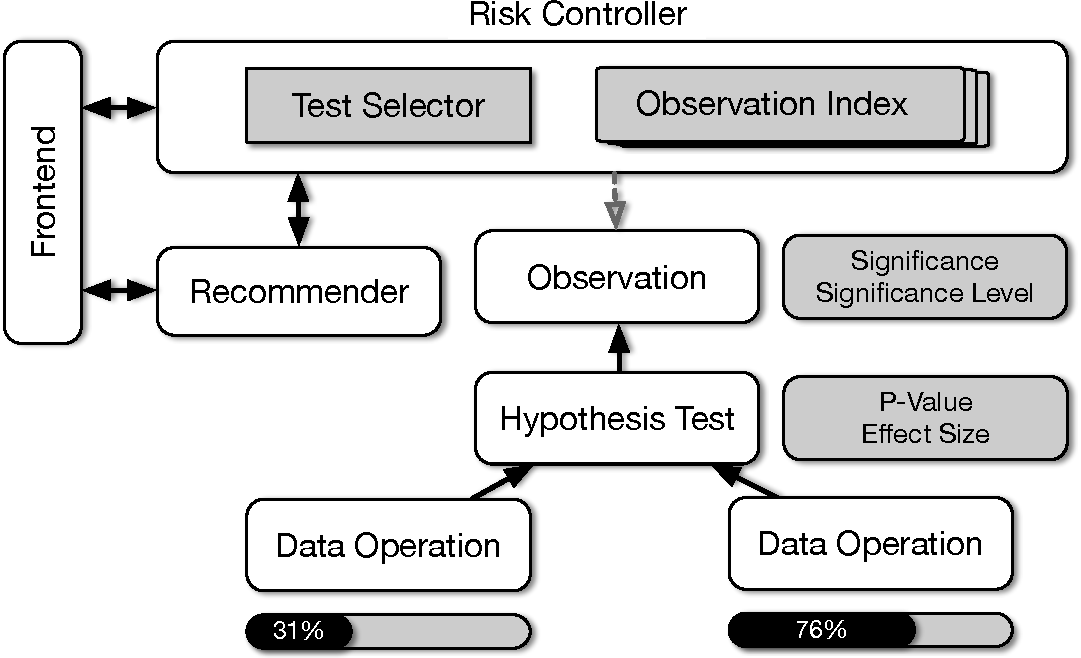
\includegraphics[width=0.43\textwidth]{figures/risk-controller.pdf}
\caption{\system{}'s backend. Uncertainties in data discovery from the user or the recommendation algorithms are automatically quantified and controlled.  Hypothesis tests are chosen automatically for usability.  Observations are tracked by the observation index to provide consistent false discovery control. The statistical computation is modeled as online aggregation for interactivity and scalability.}
\label{fig:backend}	
\vspace{-0.5ex}
\end{figure}

Several challenges exist in the design of \system{} backend.  First, to free the user from the burden of choosing appropriate hypothesis tests, we design \system{} to automatically select the appropriate testing procedures based on iput observations. The user only needs to specify via pen-\&-touch gestures what she observes, such as ``the salary distribution looks more skewed towards the higher end among male than female.''  As in Figure~\ref{fig:backend}, the \textit{risk controller} at the backend receives and decodes the observation as a corresponding null and an alternative hypothesis. Observations can also be created by the backend recommendation algorithms.  The risk controller implements the false discovery control procedures as introduced in~\cite{zhao2016controlling}, which bootstraps with an initial exploration budget and invests a fraction on each new observation.  The \textit{test selector} then chooses the appropriate test based on different criteria on the hypothesis and the data characteristics.  For example, to compare two means being different, a two-sided $t$-test is chosen; $\chi^2$-test is used to compare two histograms, but only when the frequencies are large enough; whereas for smaller frequencies, a permutation test is used. 

The second challenge is to correctly manage the past observations to provide consistent false discovery control over the time and data.  This not only has implication on performance but also on correctness for supporting multiple users and the \system{} internal recommendation engine, because repeated observations on the same data should \textit{not} be tested as different steps within a false discovery procedure~\cite{zhao2016controlling}.  As in Figure~\ref{fig:backend}, the \textit{observation index} tracks the past observations to assist the risk controller on the global decisions. A loose analogy of the observation index is perhaps a version control system, such as Git~\cite{torvalds2010git}, but in this case for observations. A side effect of such design is that it allows computing different observations in parallel, yet meanwhile enforces a linear ordering for the false discovery control procedures.

Finally, the risk control component should not incur significant overhead to impeded the interactivity of the system and the user productivity, and should scale to large datasets.  However most statistical computing tools such as R\cite{R} and MATLAB\cite{matlab} only support batch-oriented functions, so the time complexity of any derived implementation of hypothesis testing grows at least linearly in the data size.  On the other hand, computation that outputs approximate answers with online refinement proves to be most effective for user productivity~\cite{zgraggen2016progressive}. Thus to scale to large datasets while maintaining interactivity, we take a different approach by designing the statistical procedures via online aggregation~\cite{onlineagg}. In particular, the approximate hypothesis testing result is computed based on an expanding subset of the data, and output a stream of updated results to the frontend within interactive response time. The result is incrementally updated as more data is scanned, as in Figure~\ref{fig:backend}. 